\chapter{OurDirection: An Interactive Dialogue Framework}

\begin{abstract}
We propose OurDirection, an open-domain dialogue framework that is specialized in mimicking the Hansard (debate) materials from Canadian House of Commons. In this framework, we employed two sets of neural network models (Hierarchical Recurrent Encoder-Decoder (HRED) and RNNs) to generate the dialogue responses. Extensive experiments on Hansard dataset shows that the models can learn the structure of the debates, and can produce reasonable responses to the user entries. 
\end{abstract}

\section{Introduction}

Dialogue systems have boomed in recent years, e.g., Apple's Siri, Amazon's Alexa, and Google's Assistant. They have shaped a new way of human-computer interaction, where the user can accomplish certain tasks using natural language instructions. We examine the capabilities of Natural Language Generation (NLG) to produce responses that mimic the debates taking place in Parliament of Canada - House of Commons. OurDirection is open-domain dialogue system that aims to generate responses based on the actual parliamentary debates. 

The most commonly used approaches for building open-domain dialogue systems include IR models \cite{Yan2016DocChatAI} and generation models such as \cite{DBLP:journals/corr/BahdanauCB14}. The IR approach alone often fails to handle the open-domain questions where QA knowledge base is not available. We propose an open-domain framework that can be trained on debate dialogues between the members of Parliament. Our paper makes the following contributions:

\begin{itemize}
\item We curate and release the Hansard dataset based on the content of MP's debates in the House of Commons.
\item We conduct a set of experiments using different natural language generation models and evaluate the dialogue responses.
\end{itemize}


\section{OurDirection Framework}

\subsection{Hierarchical Recurrent Encoder-Decoder (HRED) response generator}
In our framework, inspired by \cite{DBLP:journals/corr/SerbanSBCP15}, we consider a dialogue as a sequence of $M$ utterances $D = \{U_1, ...., U_M\}$ between the two members of the parliament. Each $U_m$ is made of a $N_m$ tokens where $U_m = \{w_{m,1}, ... w_{m,N_m} \}$ and $W_{m,n}$ is a variable defined in the vocabulary V. The tokens used here include both words, and punctuation to preserve the structure of the natural language.  To overcome the limitations of the standard n-grams to compute the joint probabilities over the dialogues, we use an embedding layer which can be initiated with the pre-trained weights. Each column in embedding matrix is a vector representation of the token in vocabulary V. 

\textbf{Recurrent Neural Network} A recurrent neural network (RNN) is a network that operates on a sequence and can use its own outputs as an input for the subsequent steps.  An RNN models an input sequence of tokens $\{w_1, ..., w_N\}$ by means of recurrences: 
\begin{equation}
h_n = f(h_{n-1}, w_n),
\end{equation}
where \(h_n \in  \mathbb{R}^{d_n} \) is the recurrent or hidden state. The hidden state acts as a vector representation of the input tokens up to the position $n$.  An interesting property of the recurrent state is that the last state $h_N$ can be used as an order-sensitive compacted vector of the original sequence. This allows RNN to be used as an encoder in many machine learning tasks, including the language modeling. In our dialogue system, the RNN encoder maps the utterances (sentences)  to the utterance vector (Figure\ref{fig:encoder}).

 The \textit{context} RNN is a higher-level encoder that keeps track of previous utterances \cite{DBLP:journals/corr/SerbanSBCP15}.  The hidden state of context RNN can represent a reduced dimension vector of the dialogue up to the last utterance and can be used in prediction of $U_{m+1}$. Lastly, the decoder RNN is used for the prediction of the next tokens in the response. The important part of the decoder is that its predictions are conditioned on the hidden state of the context RNN, and therefore the context of the speech is preserved. The encoder, context and decoder RNN all made use of Gated Recurrent Unit (GRU) hidden units \cite{DBLP:journals/corr/BahdanauCB14}. We also used the recommended hyperbolic tangent as the activation function in all RNN layers. \vspace{-0.75em}
\begin{figure}[!ht]
	\centering
  	\caption{Encoder}
	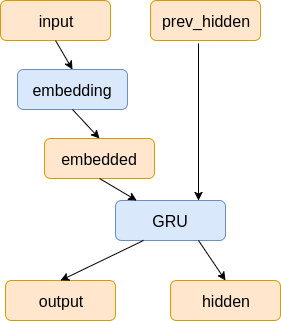
\includegraphics[scale=0.5]{img/encoder-network}
  	\label{fig:encoder}
\end{figure}

\begin{figure*}[!ht]
	\centering
  	\caption{The overall architecture of the HRED for dialogue system \cite{DBLP:journals/corr/SerbanSBCP15} }
	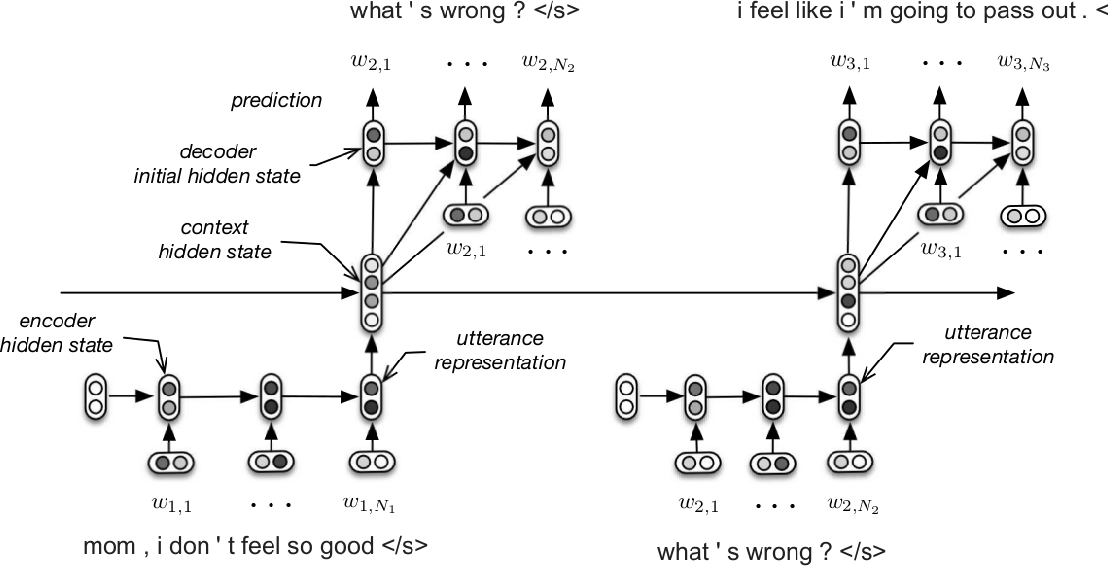
\includegraphics[width=\textwidth, height=6cm]{img/HRED}
  	\label{fig:hred}
\end{figure*}

\vspace{-0.9em}
\subsection{GRU-based Model}
In this approach, we chose to build a recurrent neural network (RNN) language model that learns the latent structure of the original text. Most of the well-known language models rely on the n-grams to highlight the latent semantics of the text. This can be a limitation since the model is built on the explicit probability of a sequence of \textit{n} words.  The RNNs, in contrast, have the ability to model longer sequences and therefore are more effective in predicting the sequences of words in sentences.  

The generative model operates slightly different than the HRED model. In this model, we use the whole question and answer text to train the model. The model tries to predict the word sequence and generate responses based on the given text. 

We designed our model as follows: the input layers take the matrix of word indices as the first layer of the model. The input layer will be fed to the embedding layer with the pre-trained weights coming from GloVe model. The recurrent GRU hidden layers are the central component of the generative model. The model will observe each token in the corpus, and use the embedding to learn the representation of the token in the sequence. We chose the GRU layer for this model. However, this layer can be changed with the Long Short-Term Memory (LSTM) unit. This first layer of GRU will return a sequence equal to the size of the input, which will be fed to second hidden layer GRU. The second recurrent layer helps us to have a deeper model which can learn the latent semantics of the text better. Lastly, to predict the probability of the next token, time distributed dense unit is used. The softmax activation function transforms the value of the hidden layers into score from 0 to 1, which can be treated as the probability of each token. The dense layer produces the probability scores for one particular position in the text sequence. The structure of the model can be seen in Figure \ref{fig:gru_generative_model}.


\vspace{-0.75em}

\begin{figure}[!ht]
	\centering
  	\caption{Language modeling for response generation}
	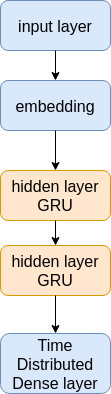
\includegraphics[scale=0.5]{img/GRU_generative}
  	\label{fig:gru_generative_model}
\end{figure}

\vspace{-0.65em}

\section{Experiments}
\subsection{Hansard Dataset}
The Canadian government has adopted the open government initiative which allows the citizens to have public access the documents and proceedings of the government. We gathered our experimental data through the open-data portals of House of Commons \footnote{https://www.ourcommons.ca/en/open-data}. More specifically, we used the Hansard (debate) records between the opposing parties. The Hansard is in intervention format, which is labeled topic discussion between two or more parliament members. The debates are usually in the form of question and answer, where the party members ask questions opposing members provide straight answers. That is sometimes, of course. Figure \ref{fig:hansard_info} shows the popularity of the discussion.

% \vspace{-0.75em}
\begin{figure}[!ht]
  	\caption{Hansard topics}
	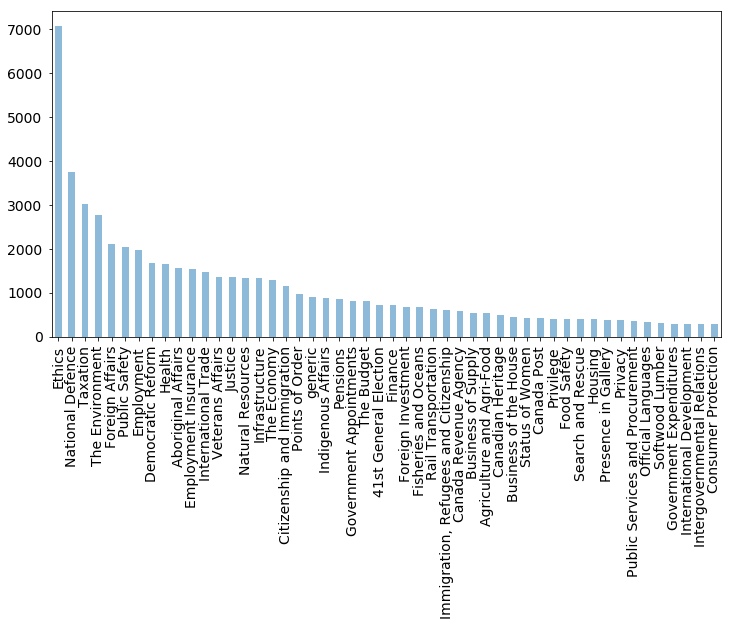
\includegraphics[width=\linewidth]{img/hansard_info}
  	\label{fig:hansard_info}
\end{figure}
% \vspace{-0.75em}

\vspace{-0.75em}

\begin{table}[ht]
% \footnotesize
\centering
\caption{Sample debate}
\label{table:debate}
\begin{tabularx}{\columnwidth}{r X}
\hline
Q & The liberal tax plan will also cost billions of dollars and will give nothing to two-thirds of Canadians. Will the government abandon its budget, which only benefits the wealthiest, and introduce a real plan for the middle class? \\ \hline
A & Mr. speaker, that is what we are doing by reducing taxes for families and increasing the child care benefit. Income splitting and the family tax cut will give nearly \$2billion to families with children.  \\ \hline
\end{tabularx}
\end{table}
\vspace{-0.75em}

We further processed the interventions to get the question and answer pairs. To cut down the size of question and answers, we only chose the last two sentences of the question and first two sentences of the answer in the final pair. This helped us to reduce the training time significantly. We observed that the actual question is usually mentioned in the last portion of question, and answers tend to wander off after two sentences. In this work, we extract debates from past three parliament session which goes back to late 2008. This process resulted in total 12,658 question/answer pairs that are used in the training of all models. Table \ref{table:debate} shows an example of question and answer in our Hansard dataset.


\subsection{Training Procedure}
The training process includes passing the input sentences through the encoder word by word, and track the output and latest hidden state. In the next step, the decoder is given the last hidden state of the context RNN as its first hidden state along with the $<SOS>$ token as it's first input. The decoder will be used in the iteration to predict the next token as described in the prediction task.

\subsubsection{Teacher Forcing and Scheduled Sampling}
This method is used to quickly and efficiently train the recurrent neural network models that use the output from one-time step (t - 1) in the sequence as an input for the next prediction \cite{DBLP:journals/corr/BengioVJS15}. This especially helps us to train and make a better prediction in sequences of text and is used in an Encoder-Decoder RNNs. To balance the effect of teacher forcing sampling, the model is trained randomly by the network output generation $50\%$ of the time. 


\subsection{Prediction Task}
\textbf{Generative models} With the model trained, we can now use it to generate new sequences of words. We compute the next word probability based on the preceding words in the question. We further improve the quality of the response generation by adjusting the normalizing factor of the predictions.  For HRED model, a beam search has been sued to approximate the probabilities of the tokens in the response. The bean search maintains the top-k (k = 5) output sequences at each prediction and results in smoother prediction. The larger $k$ size allows for multiple candidates sequences and increases the likelihood of better matching for the target sequence. However, the increase in $k$ size results in improvement of decoding speed. We also used the teacher forcing and scheduled sampling for the prediction of the HRED model. 
\vspace{-0.75em}

\subsection{Evaluation}
The evaluation of open-domain dialogue systems has proved to be a difficult problem \cite{DBLP:journals/corr/GalleyBSJAQMGD15}. In our experiments, we use four embedding-based metrics: greedy matching, embedding average, vector extrema and skip through similarity  \cite{DBLP:journals/corr/LiuLSNCP16}. The embedding-based metrics tend to be a relatively better alternative for unsupervised evaluation of generated text. The embedding-based metrics are an alternative to word-overlap based metrics (i. e. BLEU, METEOR), which consider the meaning of each generated word as defined in embedding space. The word embedding space, such as Word2Vec \cite{DBLP:mikoloveW2V} and GloVe \cite{pennington2014glove} approximate the meaning of the word by calculating the co-occurrence of the words in the corpus. 

To test the models, we chose 100 test questions and answers from the Hansard dataset unseen by the model. To evaluate the model, we use the answer from Q and A pair as a context.

\section{Discussion}
In this section the results of the experiments are presented. First, we evaluate the generated responses from the two models: HRED and GRU-based model. Table \ref{tab:evaluation} shows the evaluation results from the four embedding-based metrics. The evaluation metrics suggests that the HRED model fails to generate coherent response. We observed that the HRED model has difficulty learning longer sequences of dialogue, and can only generate limited word sequences. The GRU-base model generates better results with more comprehensible sentences. 

\begin{table*}
\centering
\caption{Dialogue response evaluation - Cosine Similarity (CS)}

\resizebox{\textwidth}{!}{%
\begin{tabular}{llll|lll}

\toprule
& \multicolumn{3}{l}{GRU-based} & \multicolumn{3}{l}{HRED} \\
& Min   & Max   & Mean   & Min    & Max    & Mean   \\
\midrule
Embedding Ave CS  &   0.759    &   0.974   &    0.907    &   0.258     &  0.813      &     0.698   \\
Skip Though CS  &   0.307    &   0.813   &    0.702    &   0.104     &   0.291     &    0.242    \\
Vector Extrema CS   &   0.217    &   0.495   &    0.352    &    0.105    &    0.429    &    0.274    \\
Greedy Matching  &   0.545    &   0.761   &    0.674    &    0.435    &     0.667   &    0.589    \\
\bottomrule

\end{tabular}
}
\label{tab:evaluation}
\end{table*}



In terms of model training performance, we can see from Figure \ref{fig:gru_generative} and \ref{fig:HRED_generative} that both models show improvements with respect to the loss function with more iterations. The improvements in GRU-based model tends to flat line, whereas the HRED loss fluctuate with downward trend.  


\begin{figure}[!ht]
    \centering
  	\caption{GRU-based model performance}
	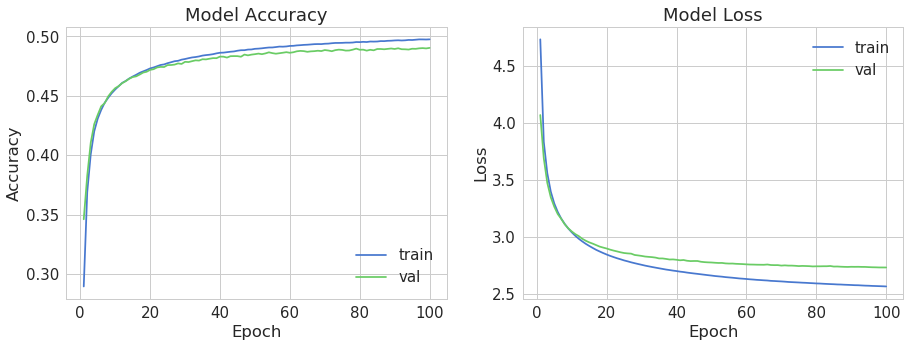
\includegraphics[width=\linewidth]{img/gru_generative}
  	\label{fig:gru_generative}
\end{figure}
\vspace{-0.9em}
\begin{figure}[!ht]
    \centering
  	\caption{HRED model - loss performance}
	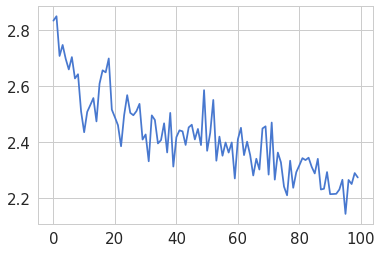
\includegraphics[scale=0.7]{img/HRED_loss}
  	\label{fig:HRED_generative}
\end{figure}

\section{Related Work}
We can categorize the problem of dialogue systems into two groups: \textit{closed-domain} and \textit{open-domain}. The closed-domain dialogue systems tend to address more specific human/machine interaction needs and are concerned with the task-based problem. These systems typically use rule-based or template-based methods to accomplish the user commands or inquiries \cite{DBLP:journals/corr/WilliamsZ16}. The open-domain systems are more diverse in their responses, and tent to be non-goal-driven. In earlier work, \cite{Ritter:2011} proposed a generative probabilistic model in the context of micro-blogs. They defined the conversation system as a translation problem, where the given text needs to be translated into the response. We also take that approach in defining the generative models to build our dialogue system.  

\section{Conclusion}
In this paper, we demonstrate the capabilities of neural networks to create a dialogue system. We first create our dialogue dataset using Canadian House of Commons open-data portals. The Hansard dataset includes the debates between the members of the parliament. After curating our dataset, we trained two sets of neural network models to generate dialogue responses based on the user given text. The results show that the models are able to learn the structure of the language (to a certain degree) and generate a response. Natural language generation is at early stages of development, and it seems to be the bottleneck for most dialogue systems. In the future, we will be using a hybrid approach to generate responses to improve on limitations of NLG and make more meaningful conversation with the user.